\documentclass[11pt,a4paper]{article}
\usepackage[margin=2.5cm]{geometry}
\usepackage{amsmath,amssymb,amsthm}
\usepackage{booktabs}
\usepackage{graphicx}
\usepackage{float}
\usepackage{hyperref}
\usepackage{fancyhdr}
\graphicspath{{../results/}}

\pagestyle{fancy}
\fancyhf{}
\fancyhead[L]{\small Markov decision processes and dynamic programming}
\fancyhead[R]{\small Risk-sensitive portfolio optimization}
\fancyfoot[C]{\thepage}
\renewcommand{\headrulewidth}{0.4pt}

\newcommand{\E}{\mathbb{E}}
\newcommand{\R}{\mathbb{R}}

\title{Risk-Sensitive Portfolio Optimization in a\\ Finite-State Markovian Environment}
\author{Xiangyu LUO \& Fangdu REN}
\date{}

\begin{document}
\maketitle
\thispagestyle{empty}

\section{Model Primitives}

The model consists of the following components:
\begin{itemize}
  \item \textbf{State process:} a finite-state Markov chain $X_t\in E=\{1,\dots,N\}$ with transition matrix $Q=(Q_{x,y})$.
  \item \textbf{Asset returns:} a risk-free asset with gross return $R_f=e^{r}$ and $m$ risky assets with a gross return vector $Z_{t+1}$. The distribution of $Z_{t+1}$ is conditioned on the state transition: $Z_{t+1}\sim\nu(x,y,dz)$ given $X_t=x$, $X_{t+1}=y$.
  \item \textbf{Action:} a vector of portfolio weights $a_t\in A\subset\R^m$, where $A$ is a compact set.
  \item \textbf{Wealth dynamics:} the portfolio wealth $V_t$ evolves according to the self-financing equation
  \[
    V_{t+1}=V_t\big[e^{r}+a_t^\top(Z_{t+1}-e^{r}\mathbf 1)\big].
  \]
\end{itemize}

\section{The Risk-Averse Problem ($\gamma>0$)}

The objective is to find a policy $\pi$ that maximizes the risk-adjusted long-run growth rate
\begin{equation}\label{eq:criterion}
  J(x,\pi)=\liminf_{T\to\infty}-\frac{2}{\gamma T}\ln\E_x^\pi\Big[\exp\Big(-\frac{\gamma}{2}\ln V_T\Big)\Big].
\end{equation}
This is equivalent to minimizing the expectation of a product of random variables:
\[
  \min_\pi\ \E_x^\pi\Big[\prod_{t=0}^{T-1}\big(e^{r}+a_t^\top(Z_{t+1}-e^{r}\mathbf 1)\big)^{-\gamma/2}\Big].
\]
A change of measure separates the one-period exponential moment from the regime dynamics, through the following components:
\begin{enumerate}
  \item \textbf{Exponential moment:}
  \[
    m_\gamma(x,a):=\sum_{y\in E}Q_{x,y}\int_{\R^m}\big(e^{r}+a^\top(z-e^{r}\mathbf 1)\big)^{-\gamma/2}\,\nu(x,y,dz).
  \]
  \item \textbf{Risk-adjusted transition kernel:}
  \[
    P^\gamma(x,a,y):=\frac{Q_{x,y}}{m_\gamma(x,a)}\int_{\R^m}\big(e^{r}+a^\top(z-e^{r}\mathbf 1)\big)^{-\gamma/2}\,\nu(x,y,dz).
  \]
  \item \textbf{Additive stage cost:}
  \[
    c_\gamma(x,a):=-\frac{2}{\gamma}\ln m_\gamma(x,a).
  \]
\end{enumerate}
With $\theta:=-\gamma/2<0$, the optimal growth rate is characterized by the multiplicative Poisson equation
\begin{equation}\label{eq:mult-poisson}
  \lambda\,w(x)=\min_{a\in A}\ m_\gamma(x,a)\sum_{y\in E}P^\gamma(x,a,y)\,w(y),\qquad w>0,\qquad \rho_\gamma=\frac{1}{\theta}\ln\lambda .
\end{equation}
Writing $w=e^{\theta h}$ and dividing the logarithm by $\theta<0$ gives
\[
  \rho_\gamma+h(x)=\max_{a\in A}\Big\{c_\gamma(x,a)+\frac{1}{\theta}\ln\sum_{y\in E}P^\gamma(x,a,y)\,e^{\theta h(y)}\Big\}.
\]
The stage term $c_\gamma$ is additive, but the continuation term is a log-sum-exp under $P^\gamma$ rather than the expectation $\sum_yP^\gamma(x,a,y)h(y)$. The change of measure therefore does not produce an ordinary (risk-neutral) average-reward MDP: the problem remains risk-sensitive, and the linear average-reward equation is recovered only in the limit $\gamma\to0$ (Section~3).

\section{The Risk-Seeking Problem ($\gamma<0$)}

For the risk-seeking case, the criterion is again a risk-sensitive long-run criterion. The objective is to find a policy $\pi$ that maximizes the long-run risk-adjusted growth rate, characterized by the ergodic dynamic programming equation. Let $h_\gamma(x)$ be the relative value function and $\rho_\gamma$ the optimal average reward (growth rate). With $\theta=-\gamma/2>0$, the Bellman equation is
\begin{equation}\label{eq:rs-bellman}
  \rho_\gamma+h_\gamma(x)=\max_{a\in A}\Big\{r(x,a)+\frac{1}{\theta}\ln\sum_{y\in E}P(y\mid x,a)\,e^{\theta h_\gamma(y)}\Big\},
\end{equation}
where $r(x,a)$ is the one-period log-return and $P(y\mid x,a)$ are the state transition probabilities. As the risk-sensitivity parameter $\gamma\to0$, a first-order Taylor expansion shows that \eqref{eq:rs-bellman} converges to the standard average-reward Bellman equation
\begin{equation}\label{eq:ar-bellman}
  \rho+h(x)=\max_{a\in A}\Big\{r(x,a)+\sum_{y\in E}P(y\mid x,a)\,h(y)\Big\}.
\end{equation}
This formulation has a span-contracting operator (under aperiodicity of the chains induced by stationary policies), ensuring convergence of standard solution algorithms like Relative Value Iteration and Policy Iteration.

\section{Relative Value Iteration for Average-Reward MDPs}

The Relative Value Iteration (RVI) algorithm solves for the differential value function in average-reward MDPs. Starting from an arbitrary $h_0$ (e.g.\ $h_0(s)=0$ for all $s$), the iteration proceeds as
\begin{equation}\label{eq:rvi}
  V_{k+1}(s)=\max_{a\in A}\Big[r(s,a)+\sum_{s'}P(s'\mid s,a)\,h_k(s')\Big],\qquad h_{k+1}(s)=V_{k+1}(s)-V_{k+1}(s_0),
\end{equation}
where $s_0$ is a fixed reference state for normalization. The process repeats until $\|h_{k+1}-h_k\|<\varepsilon$; the average reward is then $\rho=V_{k+1}(s_0)$. The corresponding optimal policy is then
\begin{equation}\label{eq:greedy}
  \pi^*(s)=\arg\max_{a\in A}\Big[r(s,a)+\sum_{s'}P(s'\mid s,a)\,h^*(s')\Big].
\end{equation}

\paragraph{Periodicity.} RVI converges when the chains induced by the stationary policies are aperiodic. On a periodic chain the normalized iterates may oscillate forever. This happens on a 3-state, 2-action toy example (action~0 moves along the cycle $0\to1\to2\to0$ with rewards $(1,0.5,0)$, action~1 stays in place with reward $0$): the optimal policy is the period-3 cycle and the span of $h_{k+1}-h_k$ stays equal to $1$, so a plain RVI loop stops at its iteration cap with a wrong $h$. The aperiodicity transform $P\leftarrow\tau I+(1-\tau)P$, $r\leftarrow(1-\tau)r$ with $\tau\in(0,1)$ leaves the optimal policies and $h$ unchanged and multiplies $\rho$ by $1-\tau$. With $\tau=0.5$, RVI converges in 39 iterations to $\rho=0.5$ and $h=(0,-0.5,-0.5)$, in agreement with Policy Iteration.

\subsection{Three-State Market Example}

Consider a market with three regimes: $S_0$ (bull), $S_1$ (neutral) and $S_2$ (bear). For a single aggressive investment action, the rewards are $r(S_0)=5$, $r(S_1)=2$, $r(S_2)=0$. The transition matrix is
\[
  P=\begin{pmatrix}0.6&0.3&0.1\\0.2&0.5&0.3\\0.1&0.3&0.6\end{pmatrix}.
\]
Iterating \eqref{eq:rvi} with reference state $S_0$ converges in 44 iterations ($\varepsilon=10^{-12}$) to
\[
  \rho=2.125,\qquad h^*=(h^*(S_0),h^*(S_1),h^*(S_2))=(0,\,-6.25,\,-10),
\]
so $h^*(S_0)>h^*(S_1)>h^*(S_2)$: the bull market state contributes the highest value to the long-run average reward. As a check, the stationary distribution of $P$ is $\mu=(0.275,0.375,0.35)$ and $\mu^\top r=2.125=\rho$.

\section{Policy Iteration for Average-Reward MDPs}

Policy Iteration alternates between two steps: policy evaluation and policy improvement.

\subsection{Two-State Investment MDP Example}

Consider a market with two states, good ($G$) and bad ($B$), and two actions, aggressive ($A$) and conservative ($C$). The reward structure is
\[
  r(G,A)=6,\quad r(G,C)=3,\quad r(B,A)=-2,\quad r(B,C)=1.
\]
The transition probabilities for action $A$ are
\[
  P(G\mid G,A)=0.7,\ P(B\mid G,A)=0.3;\qquad P(G\mid B,A)=0.4,\ P(B\mid B,A)=0.6,
\]
and for action $C$ (conservative investing makes the good regime more persistent)
\[
  P(G\mid G,C)=0.9,\ P(B\mid G,C)=0.1;\qquad P(G\mid B,C)=0.3,\ P(B\mid B,C)=0.7.
\]

\paragraph{Policy evaluation.} Given a policy $\pi$, we solve the system of linear equations for the average reward $\rho$ and the relative values $h(s)$:
\begin{align*}
  \rho+h(G)&=r(G,\pi(G))+P(G\mid G,\pi(G))\,h(G)+P(B\mid G,\pi(G))\,h(B),\\
  \rho+h(B)&=r(B,\pi(B))+P(G\mid B,\pi(B))\,h(G)+P(B\mid B,\pi(B))\,h(B).
\end{align*}
Setting one relative value to a constant (e.g.\ $h(B)=0$) makes the system solvable.

\paragraph{Policy improvement.} With the computed values $h(s)$, the policy is updated for each state $s$:
\[
  \pi'(s)=\arg\max_{a\in A}\Big[r(s,a)+\sum_{s'}P(s'\mid s,a)\,h(s')\Big].
\]
The process is repeated until the policy no longer changes between iterations.

\paragraph{Result.} Starting from $\pi_0=(C,C)$, evaluation gives $\rho=2.5$ and $h=(5,0)$; the improvement step switches to $A$ in the good state, and the evaluation of $\pi_1=(A,C)$ gives $\rho=3.5$, $h=(25/3,0)$. The next improvement step leaves the policy unchanged, so Policy Iteration stops after two evaluations with $\pi^*=(A,C)$: invest aggressively in the good regime and conservatively in the bad one. Relative Value Iteration returns the same policy and $\rho$. Table~\ref{tab:policies} lists the average rewards of all four stationary policies, and Figure~\ref{fig:two-state} shows the two transition structures.

\begin{table}[H]
\centering
\caption{Average reward of the four stationary policies of the two-state investment MDP.}
\label{tab:policies}
\begin{tabular}{lcccc}
\toprule
Policy $(\pi(G),\pi(B))$ & $(A,A)$ & $(A,C)$ & $(C,A)$ & $(C,C)$\\
\midrule
$\rho^\pi$ & 2.5714 & \textbf{3.5000} & 2.0000 & 2.5000\\
\bottomrule
\end{tabular}
\end{table}

\begin{figure}[H]
\centering
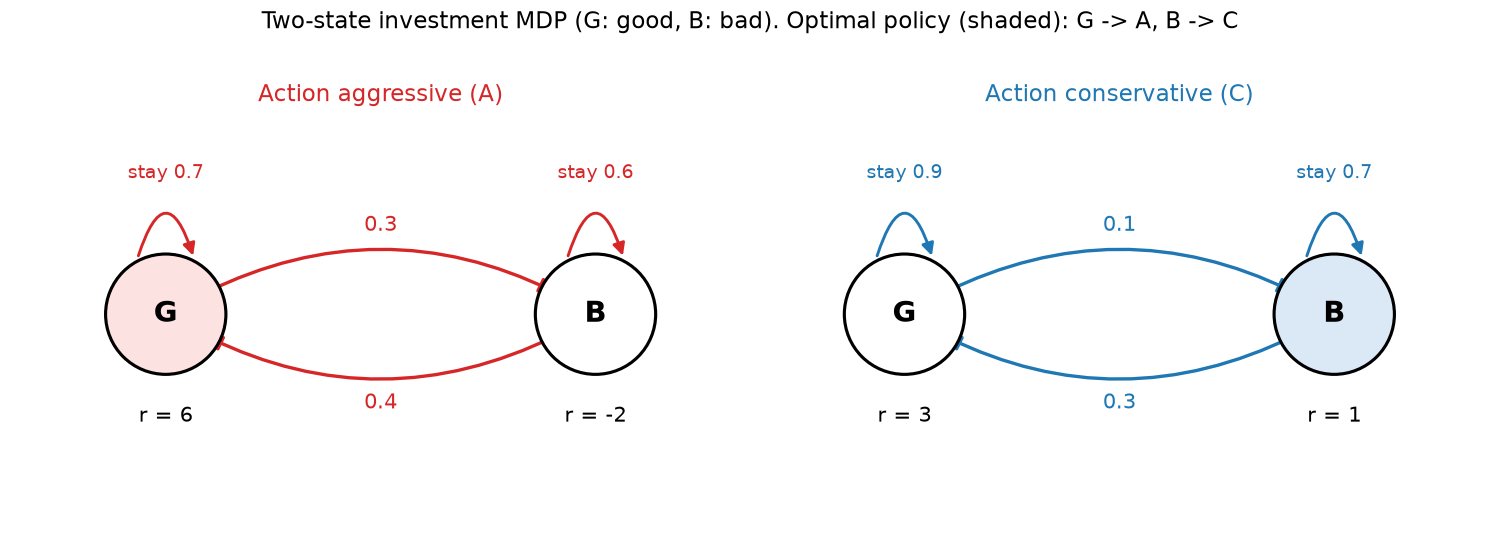
\includegraphics[width=0.95\linewidth]{two_state_mdp.png}
\caption{Two-state investment MDP under the aggressive (left) and conservative (right) actions; shaded states mark the optimal action.}
\label{fig:two-state}
\end{figure}

\section{Numerical Study of the Risk-Sensitive Portfolio}

We now solve the risk-sensitive portfolio problem of Sections~1--3 numerically for a single risky asset ($m=1$).

\paragraph{Market.} The regime chain is the three-state market of Section~4.1 (bull, neutral, bear) with transition matrix $Q=P$. Time is measured in months, the risk-free log-rate is $r=0.002$, and the risky gross return depends on the regime reached at the end of the period: $\ln Z\mid(x,y)\sim\mathcal N(\mu_y,\sigma_y^2)$ with $\mu=(0.020,\,0.008,\,-0.015)$ and $\sigma=(0.035,\,0.045,\,0.075)$ for (bull, neutral, bear). The integrals against $\nu$ are computed with a 9-point Gauss--Hermite rule, and the allocation set is the grid $A=\{0,0.01,\dots,1.5\}$ (leverage up to $1.5$; wealth stays positive at every quadrature node).

\paragraph{Ergodic equation.} With $\theta:=-\gamma/2$ and $G(a,z)=e^{r}+a(z-e^{r})$, the criterion \eqref{eq:criterion} leads, in growth units, to
\begin{equation}\label{eq:num-bellman}
  \rho_\gamma+h(x)=\max_{a\in A}\ \frac{1}{\theta}\ln\sum_{y\in E}Q_{x,y}\,\E\big[G(a,Z)^{\theta}\mid x,y\big]\,e^{\theta h(y)} .
\end{equation}
For $\gamma>0$ ($\theta<0$), maximizing the right-hand side is minimizing the exponential moment, i.e.\ \eqref{eq:num-bellman} is the multiplicative Poisson equation~\eqref{eq:mult-poisson} of Section~2 written for $w=e^{\theta h}$, with $\rho_\gamma=-\frac{2}{\gamma}\ln\lambda$ for its eigenvalue $\lambda$. For $\gamma<0$ it is equation~\eqref{eq:rs-bellman} with the random one-period log-return kept inside the exponential. As $\gamma\to0$ it reduces to \eqref{eq:ar-bellman} with $r(x,a)=\sum_yQ_{x,y}\E[\ln G(a,Z)\mid x,y]$. We solve \eqref{eq:num-bellman} with RVI (reference state: bull, tolerance $10^{-12}$; 31--37 iterations).

\paragraph{Verification.} Every optimal stationary policy $a^*(\cdot)$ is evaluated independently: its risk-sensitive growth rate equals $\frac1\theta\ln\lambda_{\mathrm{PF}}(K)$, where $\lambda_{\mathrm{PF}}$ is the Perron--Frobenius eigenvalue of the twisted kernel $K(x,y)=Q_{x,y}\,\E[G(a^*(x),Z)^{\theta}\mid x,y]$ (stationary-distribution average of $r$ for $\gamma=0$). This value agrees with the RVI value $\rho_\gamma$ to $10^{-12}$ for every $\gamma$. In addition, a $200\,000$-month simulation of the risk-neutral optimal policy gives an average log-growth of $0.006919\pm0.000217$ (95\% confidence interval), consistent with $\rho_0=0.006839$. Finally, $\rho_{-0.1}=0.006908$ and $\rho_{0.1}=0.006774$ bracket $\rho_0$, as expected from the continuity of \eqref{eq:num-bellman} in $\gamma$.

\paragraph{Results.} Table~\ref{tab:rs} and Figure~\ref{fig:rs} report the optimal allocations and growth rates. In every case the investor holds no risky asset in the bear regime and is fully levered in the bull regime unless risk aversion is strong. The neutral regime, where the expected excess return is small relative to the volatility, carries the trade-off: the allocation decreases monotonically from the leverage cap for risk-seeking investors ($\gamma\le-1$) to $0.98$ for the log-optimal (Kelly) investor and $0.10$ for $\gamma=16$. Risk aversion beyond $\gamma\approx4$ also cuts the bull-regime exposure ($1.08$ at $\gamma=8$, $0.60$ at $\gamma=16$). The optimal risk-adjusted growth rate $\rho_\gamma$ is decreasing in $\gamma$, from $13.1\%$ per year at $\gamma=-4$ to $8.2\%$ for the risk-neutral criterion and $3.6\%$ at $\gamma=16$: the risk-averse investor gives up expected growth in exchange for a lower dispersion of $\ln V_T$.

\begin{table}[H]
\centering
\caption{Optimal stationary allocations $a^*(x)$ and risk-adjusted growth $\rho_\gamma$.}
\label{tab:rs}
\begin{tabular}{rcccc}
\toprule
$\gamma$ & $a^*(\text{bull})$ & $a^*(\text{neutral})$ & $a^*(\text{bear})$ & $\rho_\gamma$ (\% / year)\\
\midrule
$-4$ & 1.50 & 1.50 & 0 & 13.14\\
$-1$ & 1.50 & 1.50 & 0 & 9.29\\
$-0.5$ & 1.50 & 1.31 & 0 & 8.67\\
$0$ & 1.50 & 0.98 & 0 & 8.21\\
$0.5$ & 1.50 & 0.78 & 0 & 7.84\\
$1$ & 1.50 & 0.64 & 0 & 7.53\\
$2$ & 1.50 & 0.48 & 0 & 6.98\\
$4$ & 1.50 & 0.31 & 0 & 6.01\\
$8$ & 1.08 & 0.18 & 0 & 4.61\\
$16$ & 0.60 & 0.10 & 0 & 3.63\\
\bottomrule
\end{tabular}
\end{table}

\begin{figure}[H]
\centering
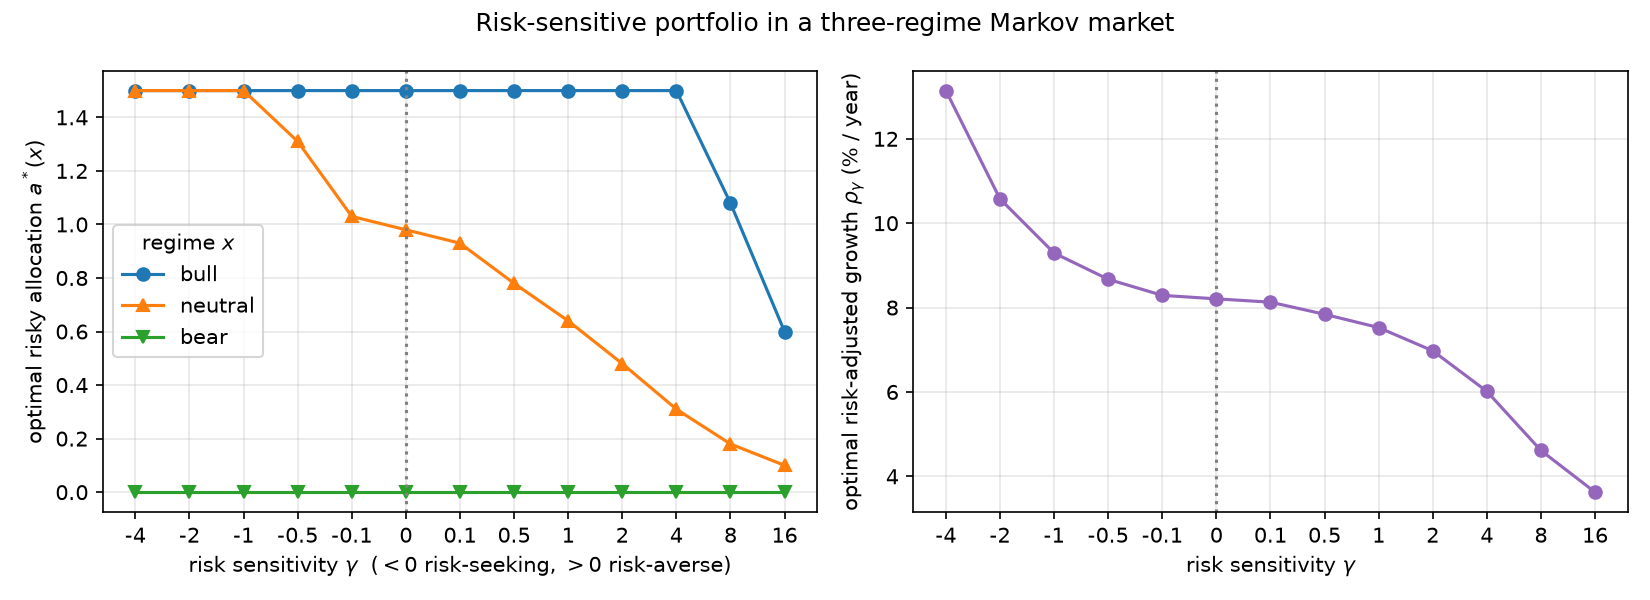
\includegraphics[width=\linewidth]{risk_sensitive_sweep.png}
\caption{Optimal allocation per regime (left) and optimal risk-adjusted growth rate (right) as functions of the risk-sensitivity parameter $\gamma$.}
\label{fig:rs}
\end{figure}

\section{Conclusion}

The risk-sensitive growth criterion turns the multiplicative wealth dynamics into an ergodic Bellman equation which, for a finite-state Markov market, can be solved with the same relative value and policy iteration schemes as risk-neutral average-reward MDPs. The examples show the practical points of these algorithms (normalization, aperiodicity, finite convergence of Policy Iteration), and the portfolio study shows how the risk-sensitivity parameter reshapes the regime-dependent allocation: risk aversion first removes exposure in ambiguous regimes, then in favourable ones.

\appendix
\section{Code}

The code is available in the accompanying folder:
\begin{itemize}
  \item \texttt{mdp\_average\_reward.py} --- Relative Value Iteration (with optional aperiodicity transform), policy evaluation and Policy Iteration; runs the three examples of Sections~4--5 and draws Figure~\ref{fig:two-state}.
  \item \texttt{risk\_sensitive\_portfolio.py} --- discretization of the market, RVI for \eqref{eq:num-bellman}, Perron--Frobenius and Monte Carlo checks, and the $\gamma$ sweep of Section~6 (Table~\ref{tab:rs}, Figure~\ref{fig:rs}).
\end{itemize}

\end{document}
